\chapter{Results}
\section{Forward Map}
\subsection{DAG}

\subsection{Bayesian Model and prior analysis}

\section{Affine Map}
\subsection{First MTC}
\subsubsection{Marginal Posterior}

\begin{figure}[ht!]
	\centering
	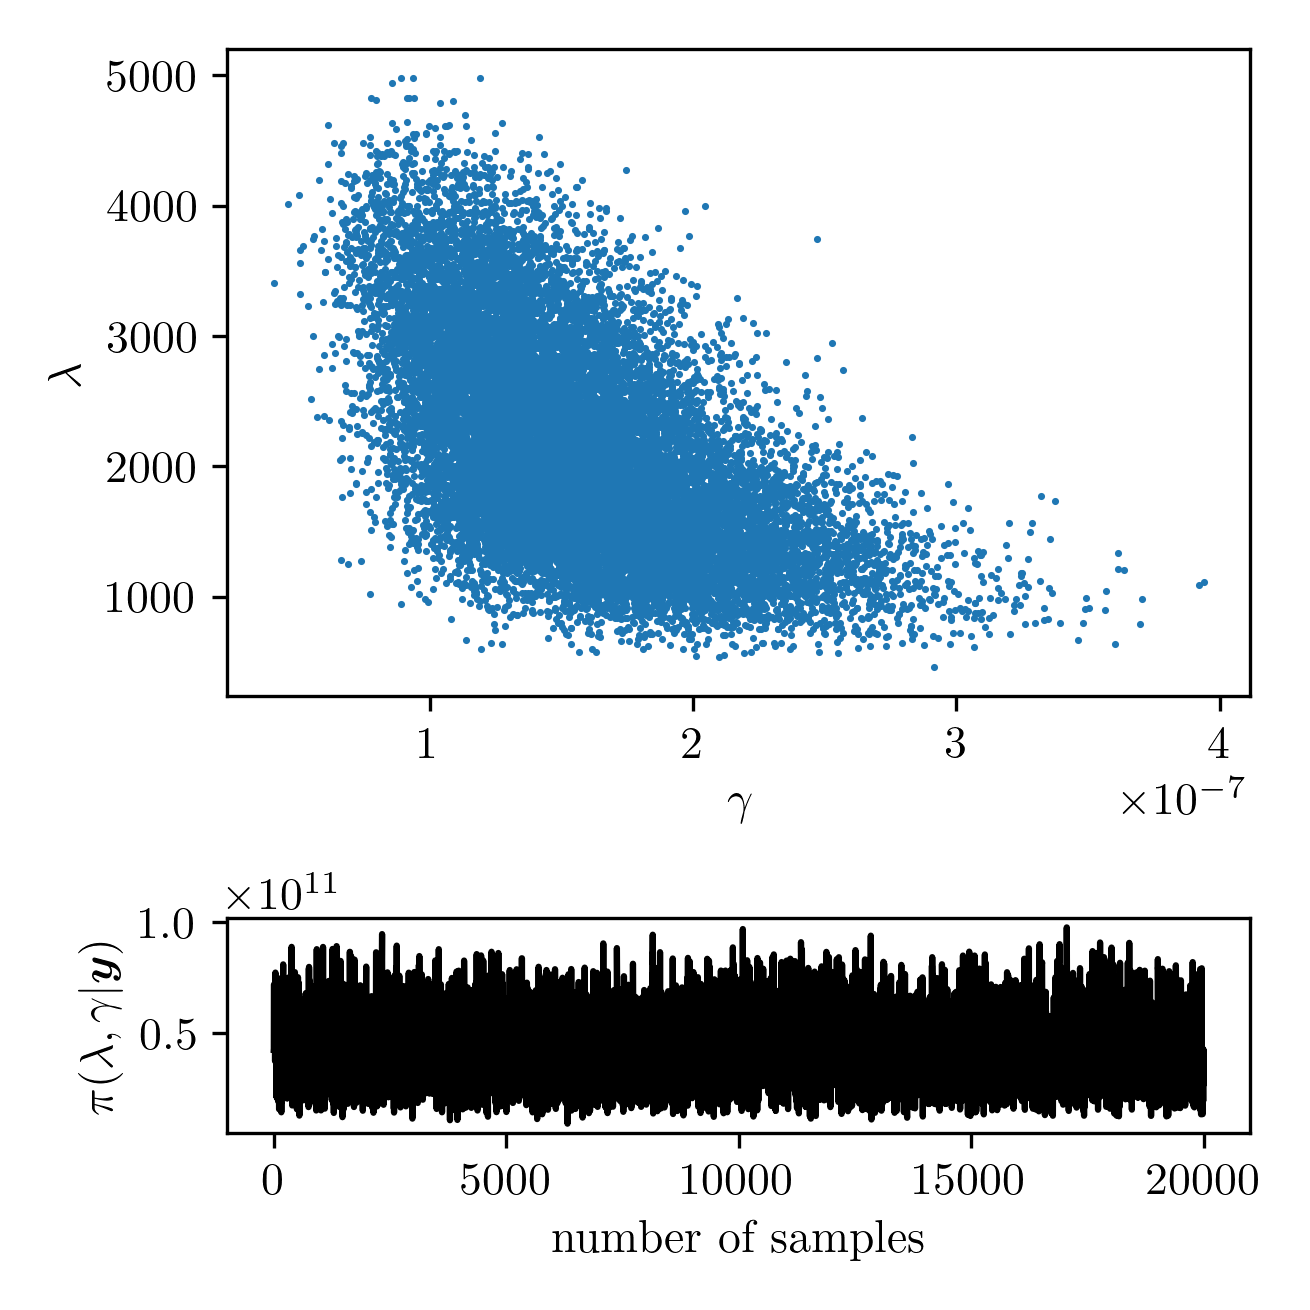
\includegraphics{ScatterplusHisto.png}
	\caption[]{}
	\label{fig:}
\end{figure}

\begin{figure}[ht!]
	\centering
	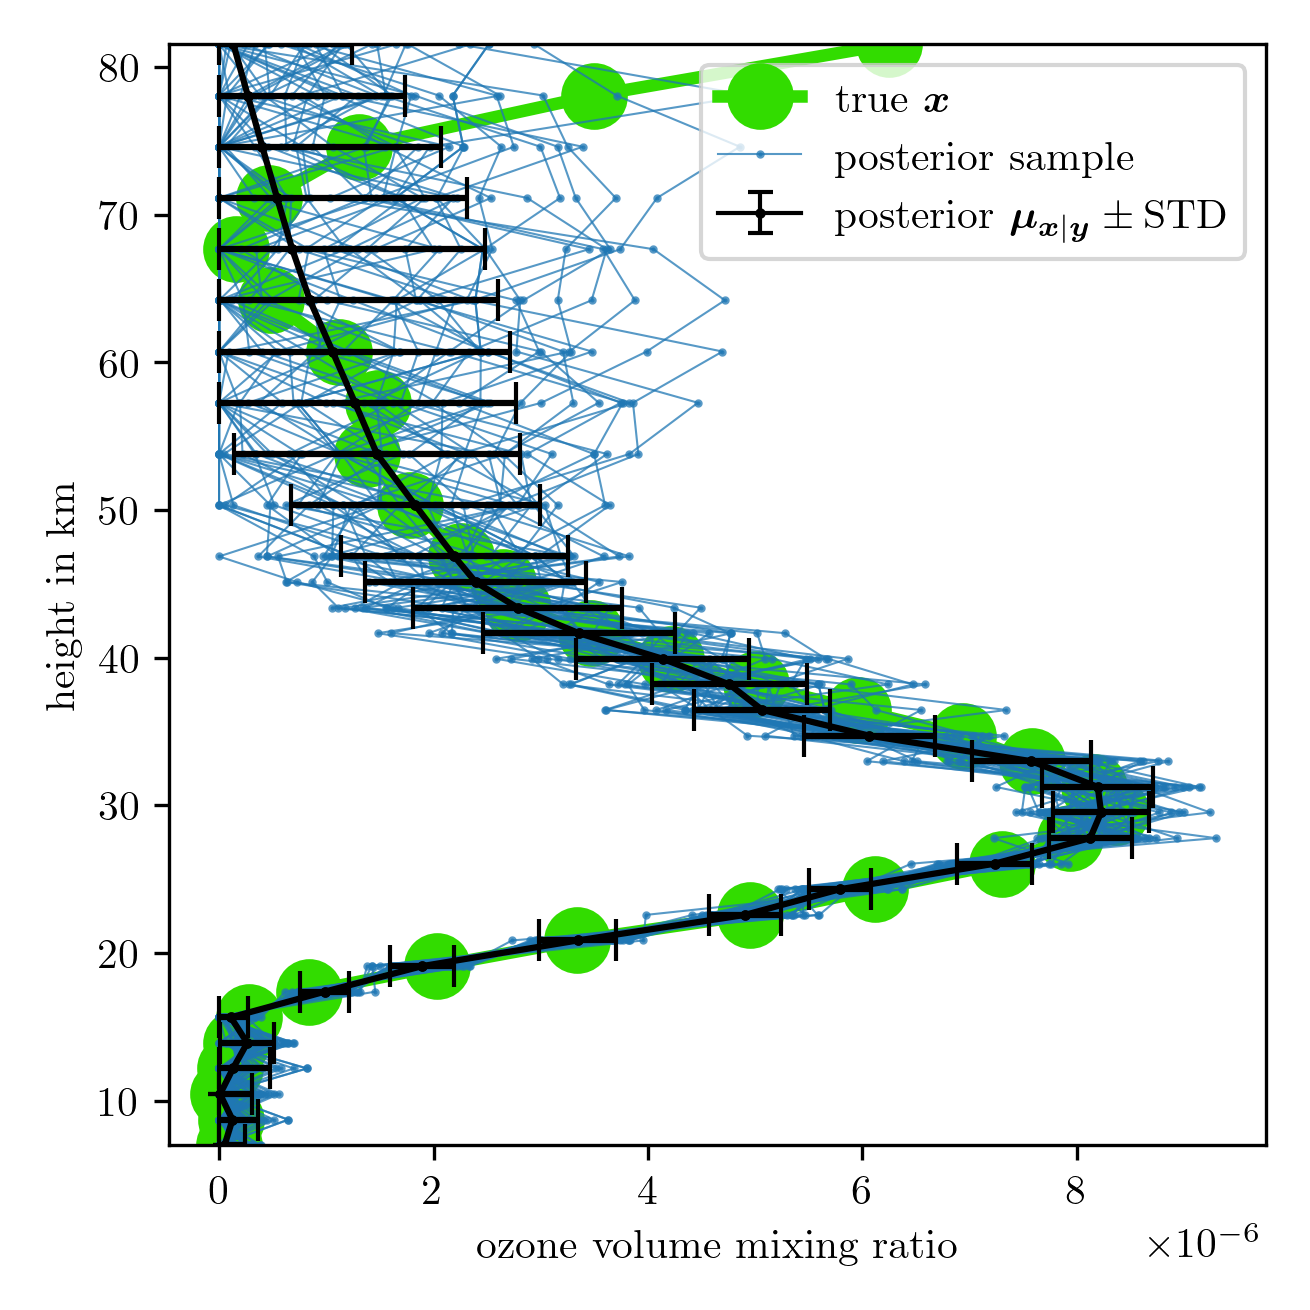
\includegraphics{FirstTestRes.png}
	\caption[]{}
	\label{fig:}
\end{figure}


\subsection{Asses Affine Map}
\begin{figure}[ht!]
	\centering
	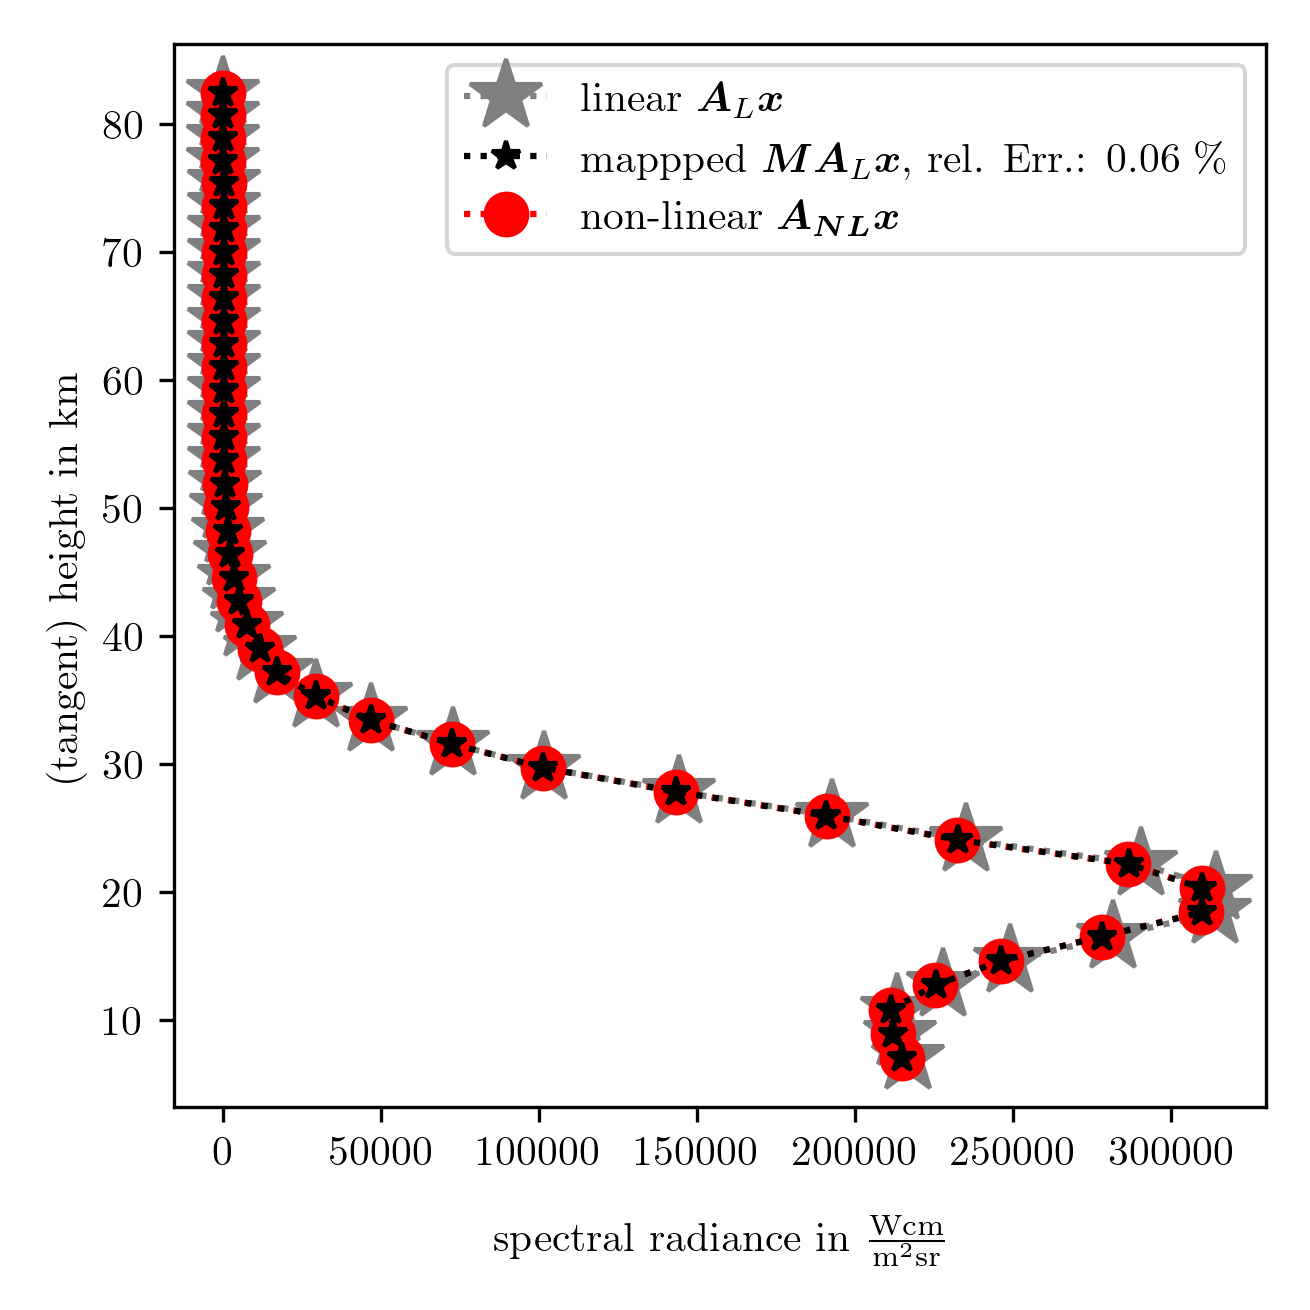
\includegraphics{SampMapAssesment.png}
	\caption[]{}
	\label{fig:}
\end{figure}
\section{Ozone Retrieval }
\begin{figure}[ht!]
	\centering
	\includegraphics{secRecRes.png}
	\caption[]{}
	\label{fig:}
\end{figure}

\subsection{Marginal Posterior}
\begin{figure}[ht!]
	\centering
	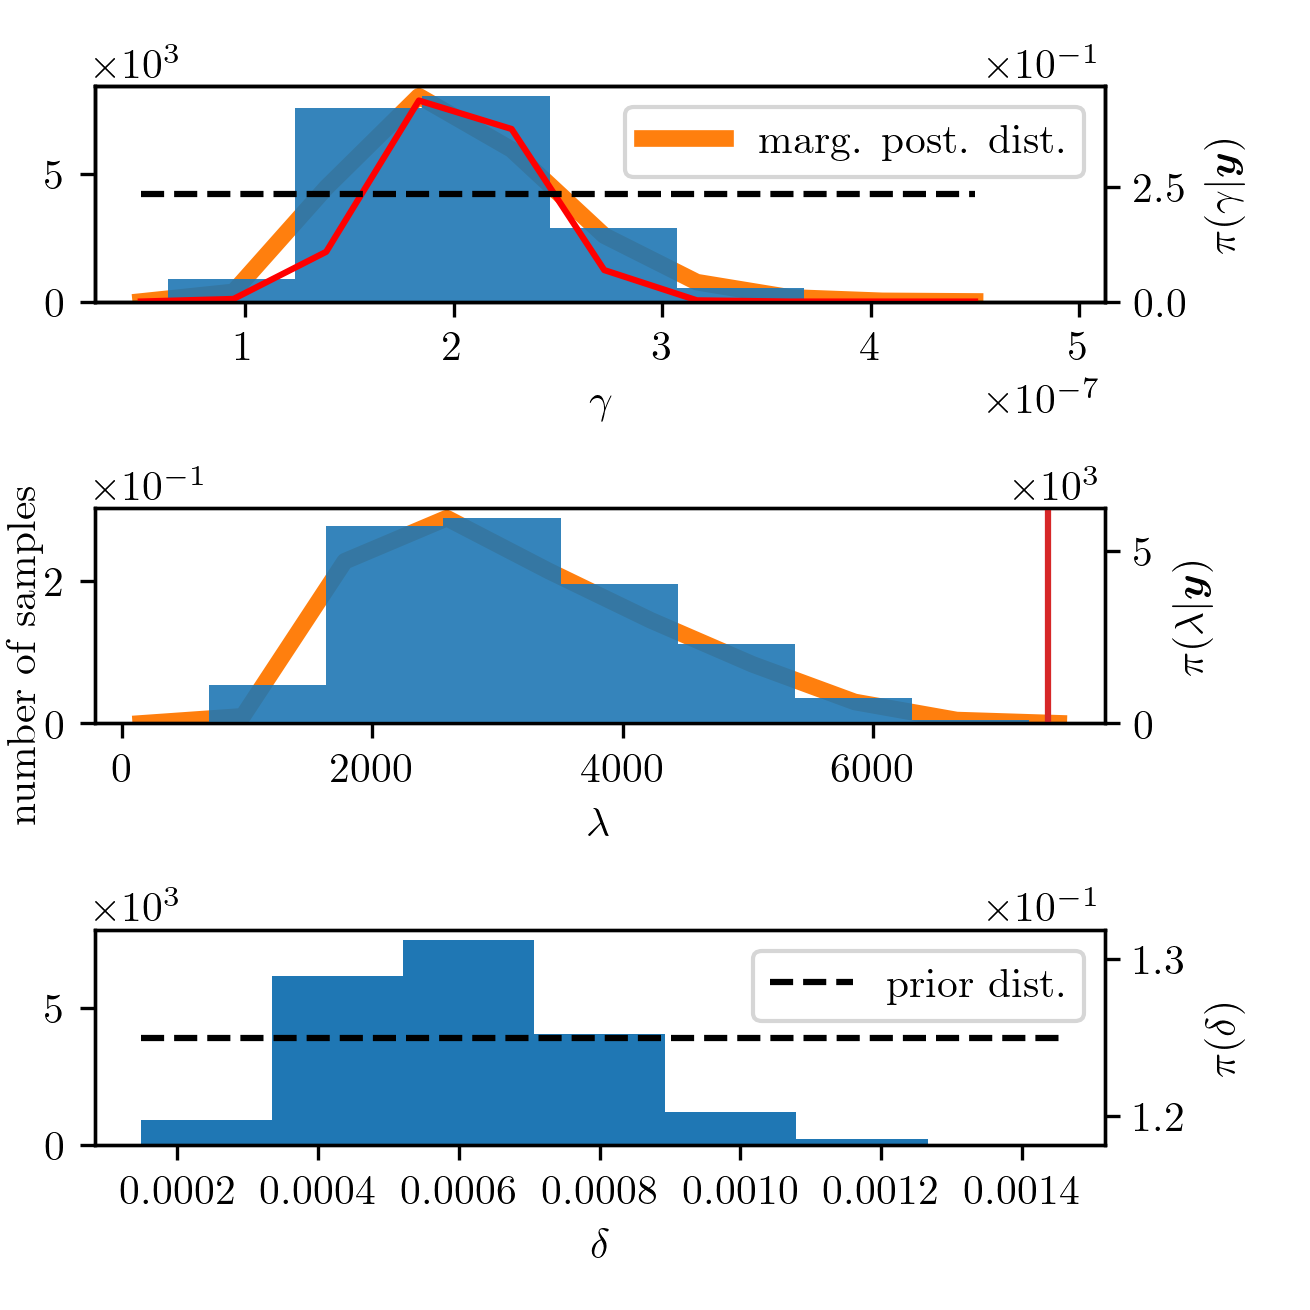
\includegraphics{secSIRTMargMargO3Res.png}
	\caption[]{}
	\label{fig:}
\end{figure}
\subsection{Regularized Solution}

\begin{figure}[ht!]
	\centering
	\includegraphics{Reg.png}
	\caption[]{}
	\label{fig:}
\end{figure}
\section{Posterior Pressure and Temperature}
\begin{figure}[ht!]
	\centering
	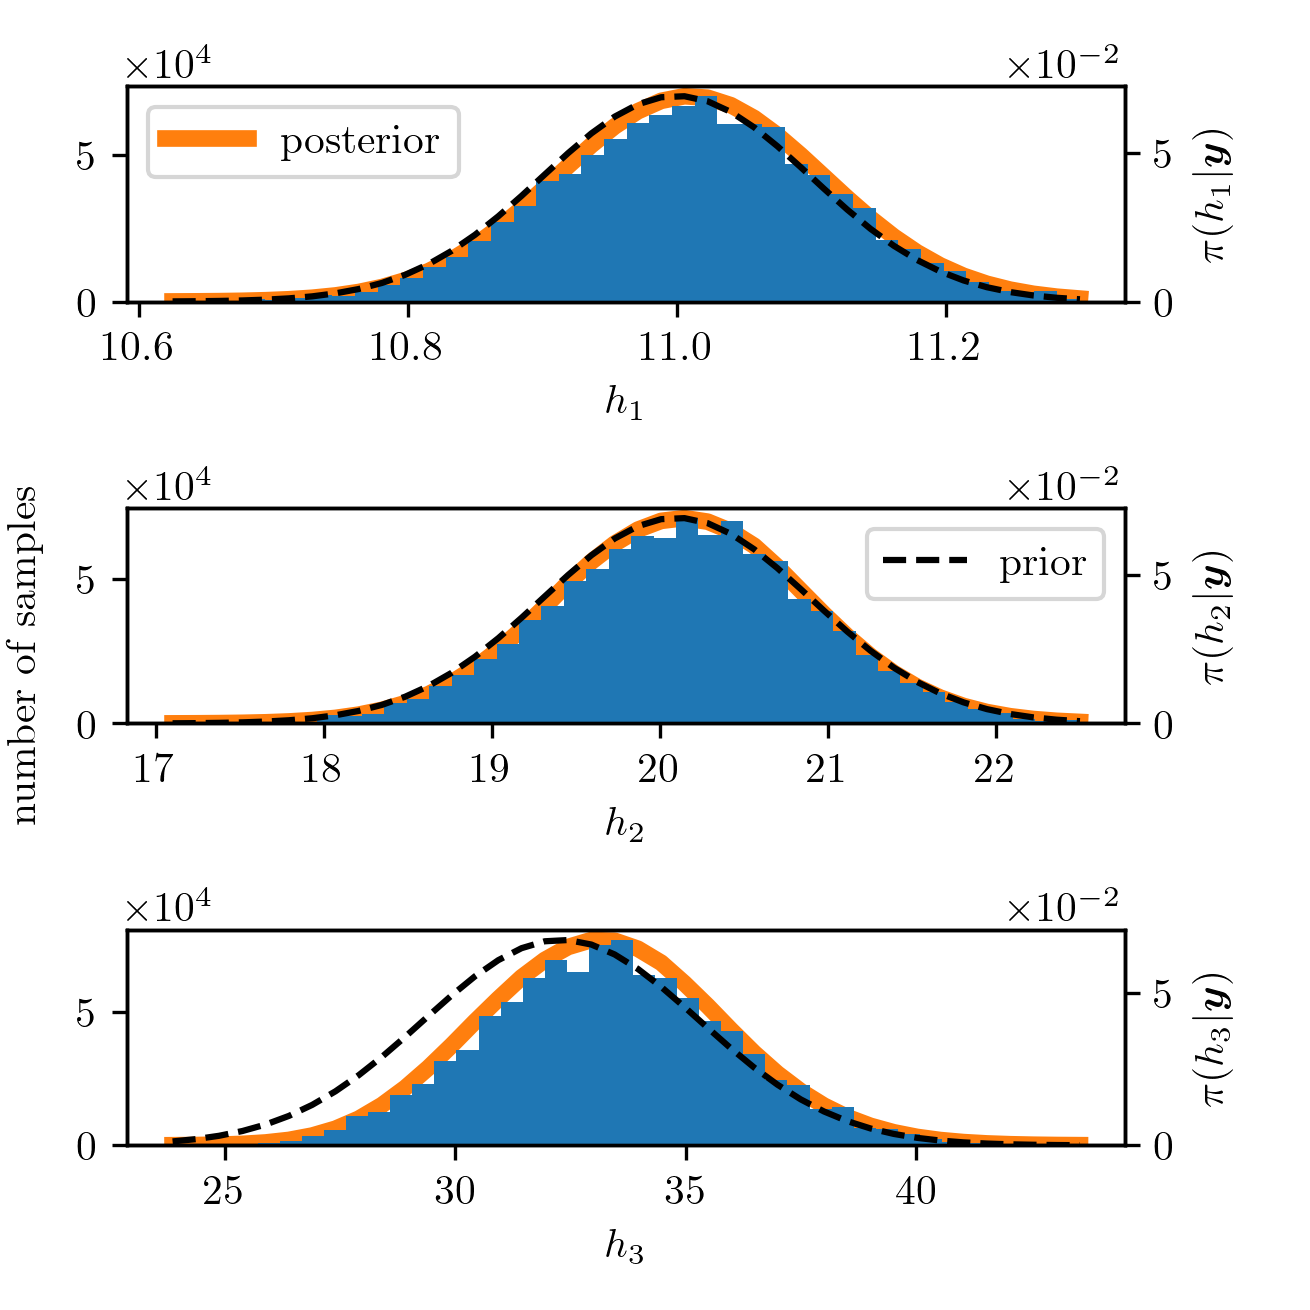
\includegraphics{PHdPTPost0.png}
	\caption[]{}
	\label{fig:}
\end{figure}
\begin{figure}[ht!]
	\centering
	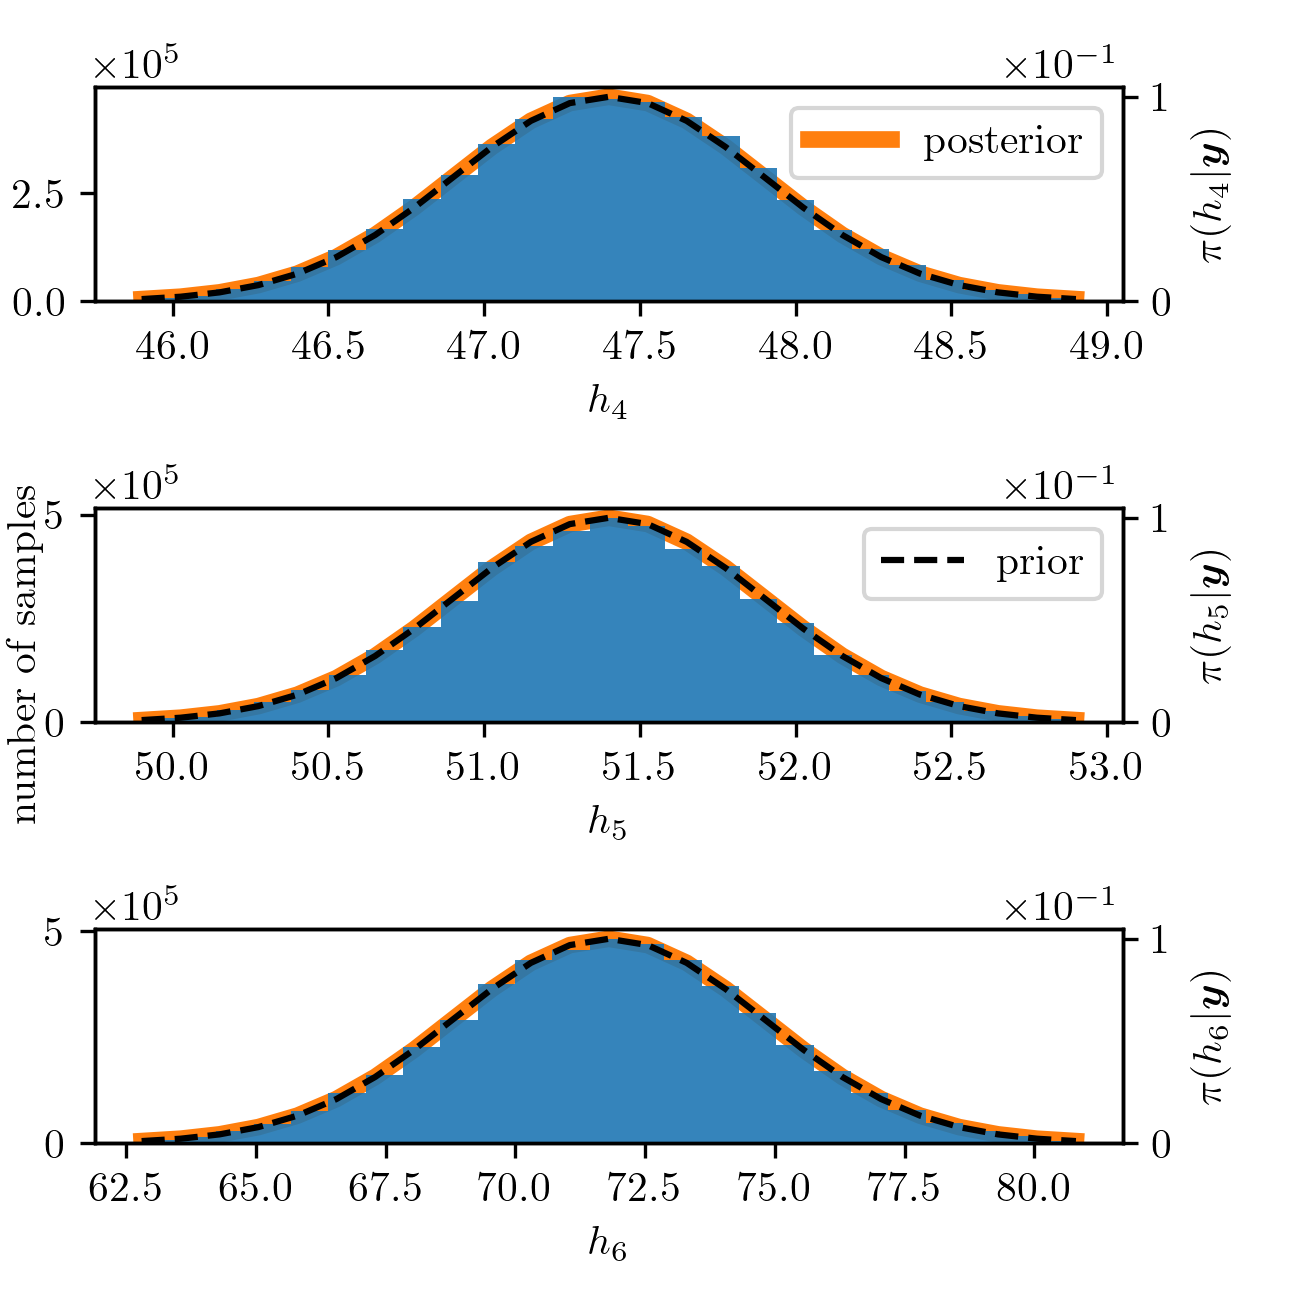
\includegraphics{PHdPTPost1.png}
	\caption[]{}
	\label{fig:}
\end{figure}
\begin{figure}[ht!]
	\centering
	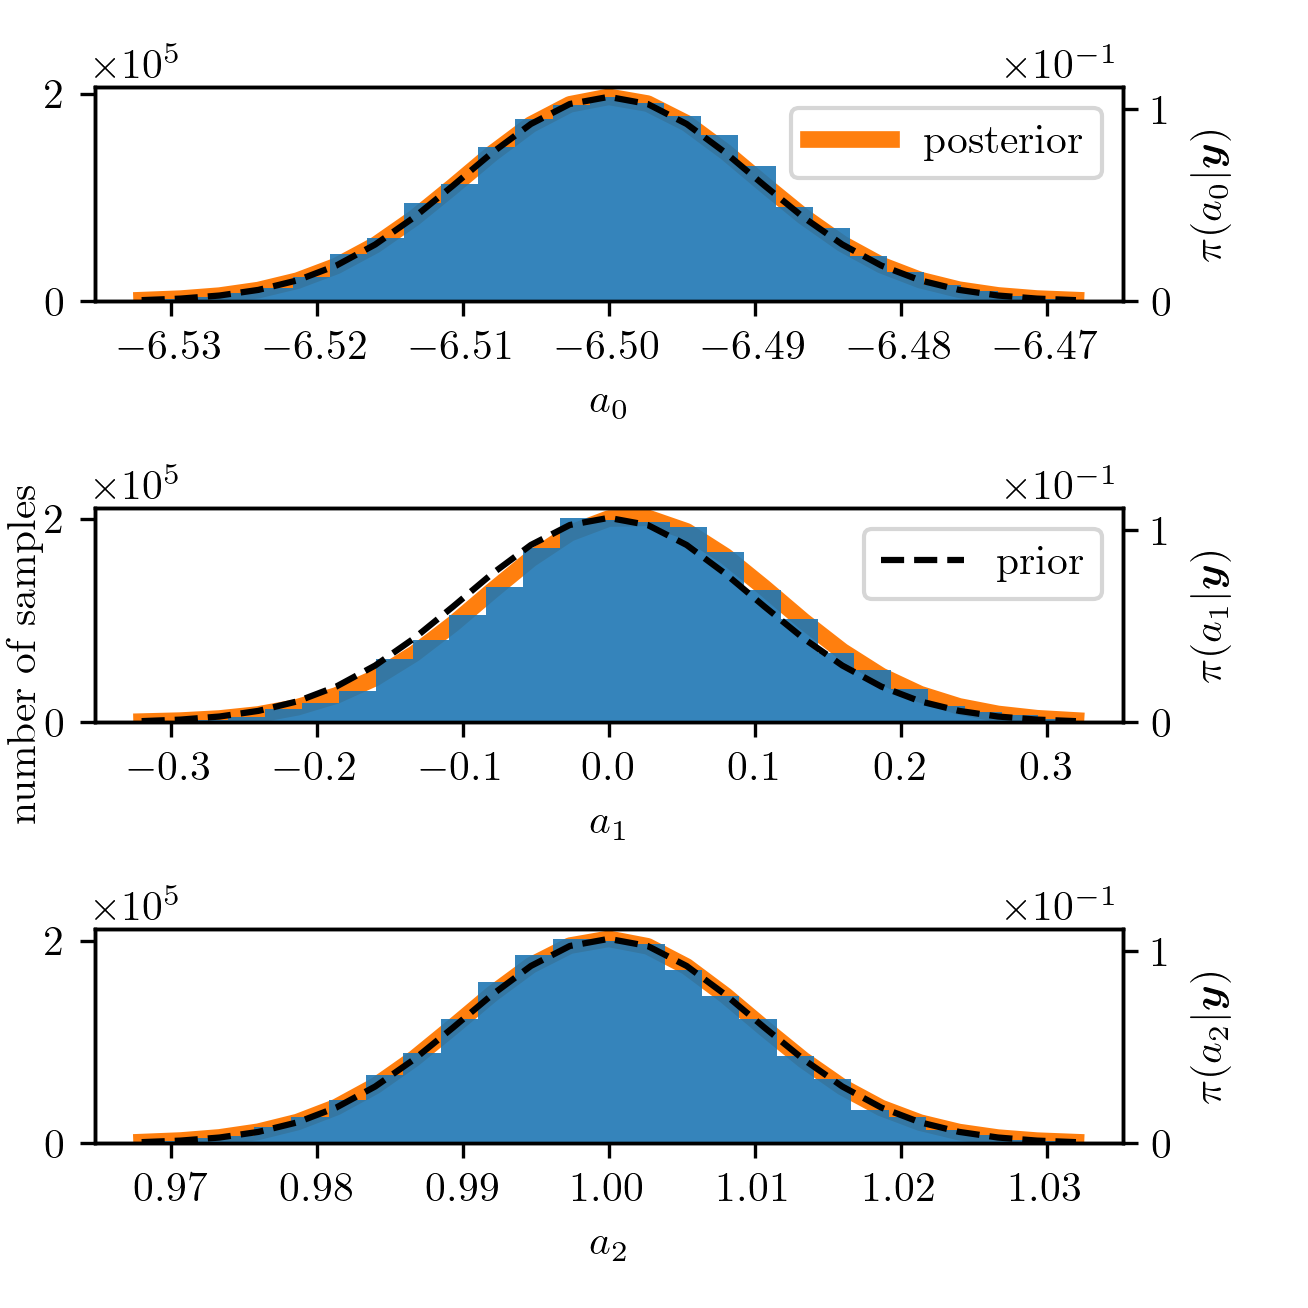
\includegraphics{PHdPTPost2.png}
	\caption[]{}
	\label{fig:}
\end{figure}
\begin{figure}[ht!]
	\centering
	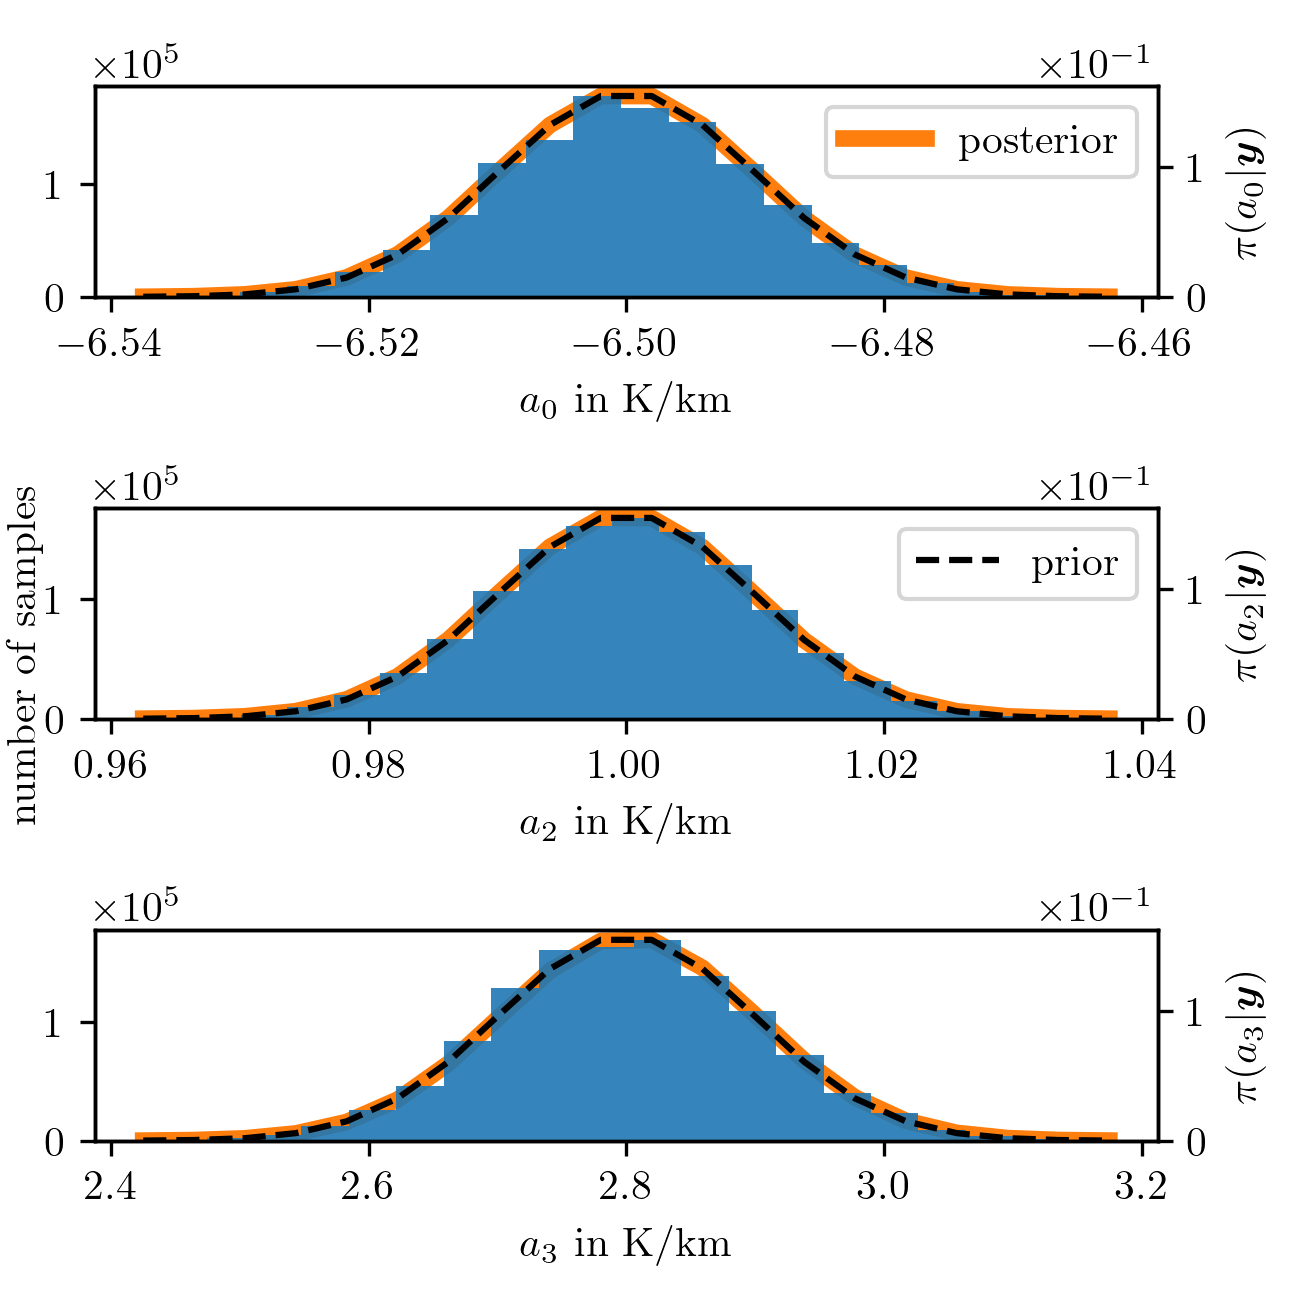
\includegraphics{PHdPTPost3.png}
	\caption[]{}
	\label{fig:}
\end{figure}
\begin{figure}[ht!]
	\centering
	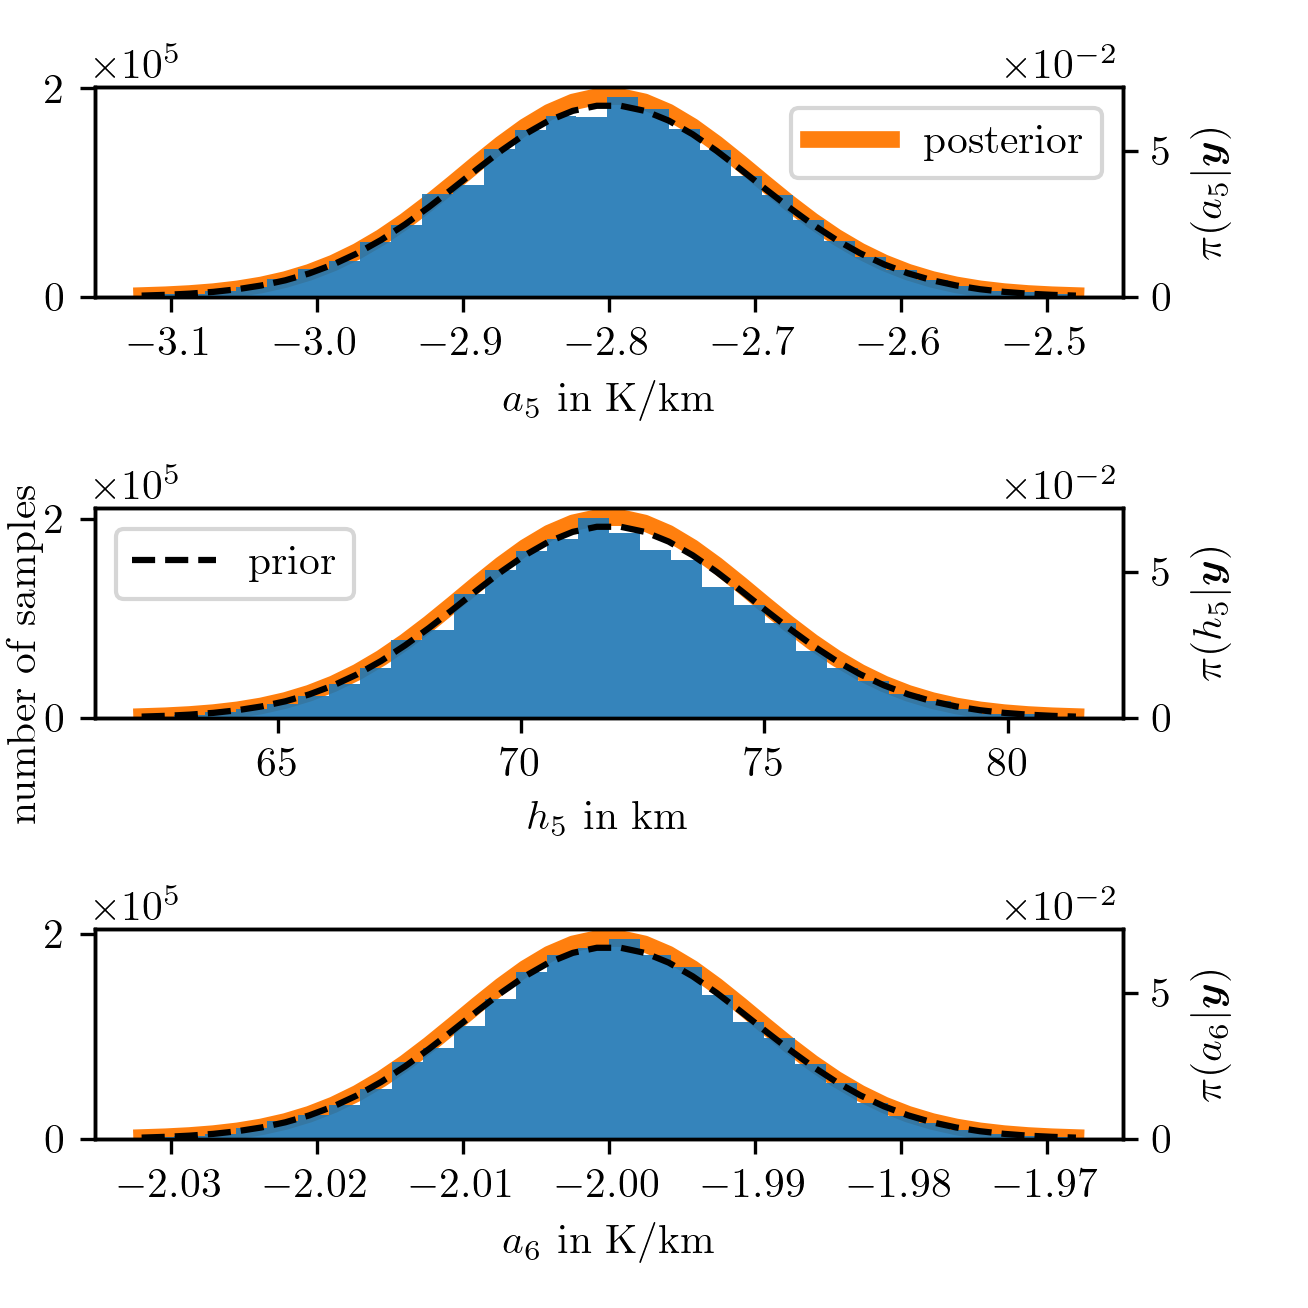
\includegraphics{PHdPTPost4.png}
	\caption[]{}
	\label{fig:}
\end{figure}

\begin{figure}[ht!]
	\centering
	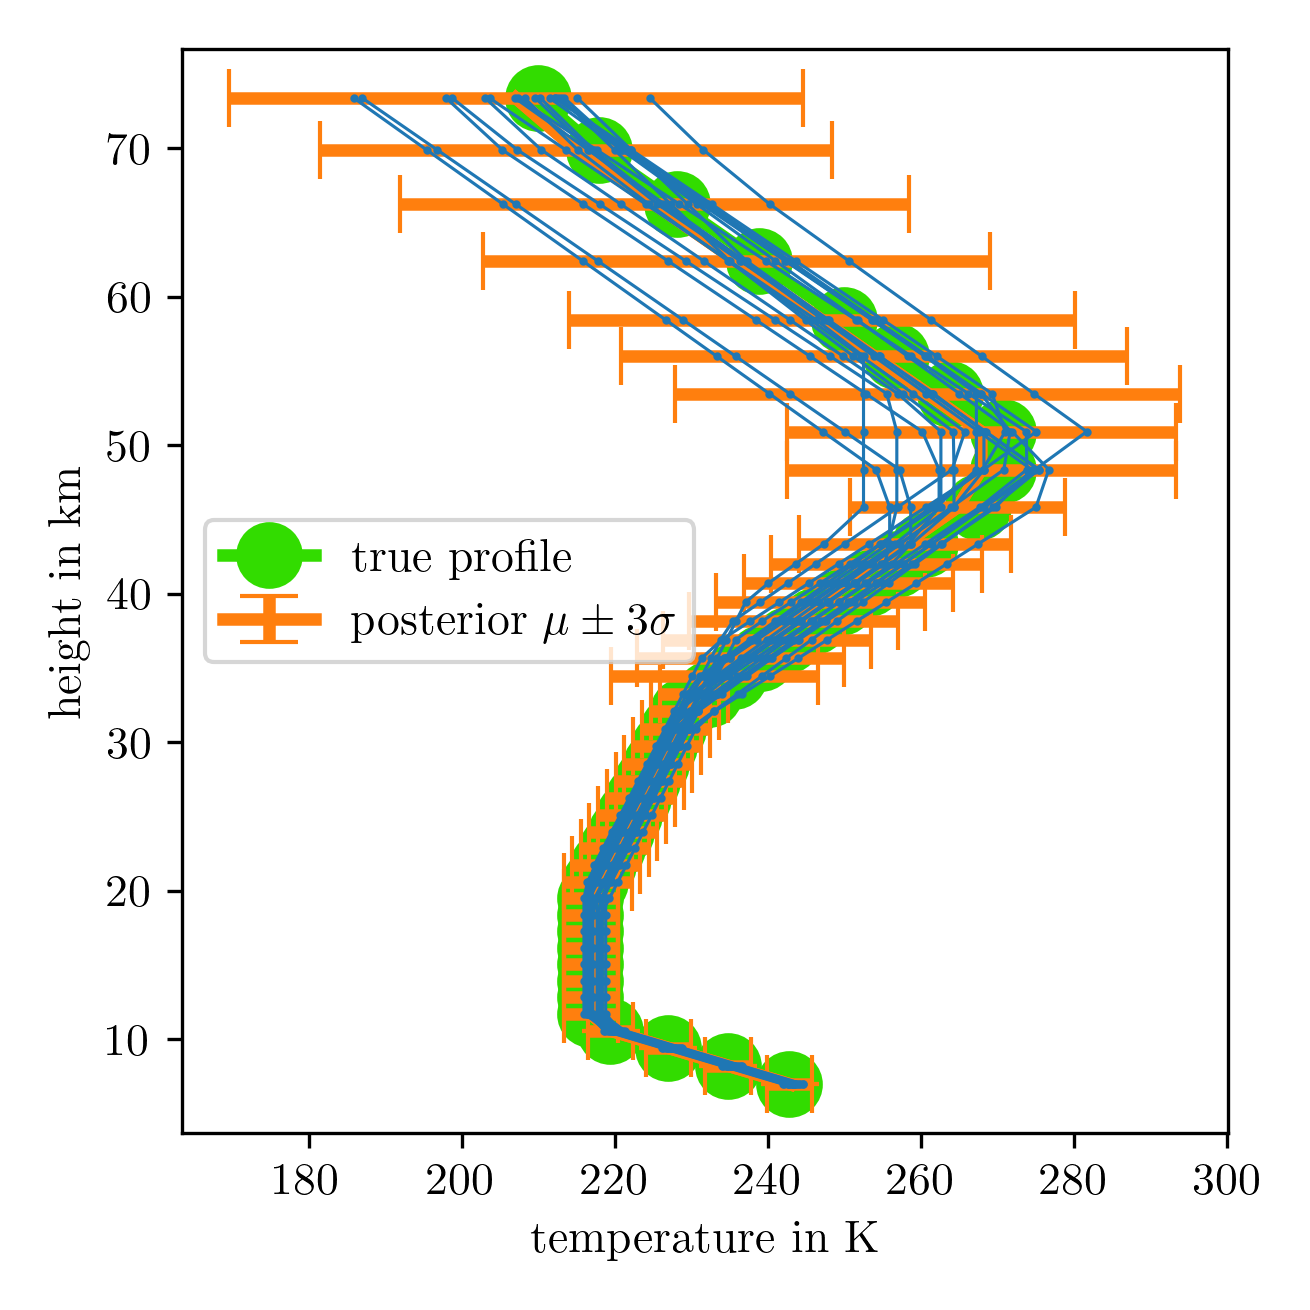
\includegraphics{TempPostMeanSigm.png}
	\caption[]{}
	\label{fig:}
\end{figure}

\begin{figure}[ht!]
	\centering
	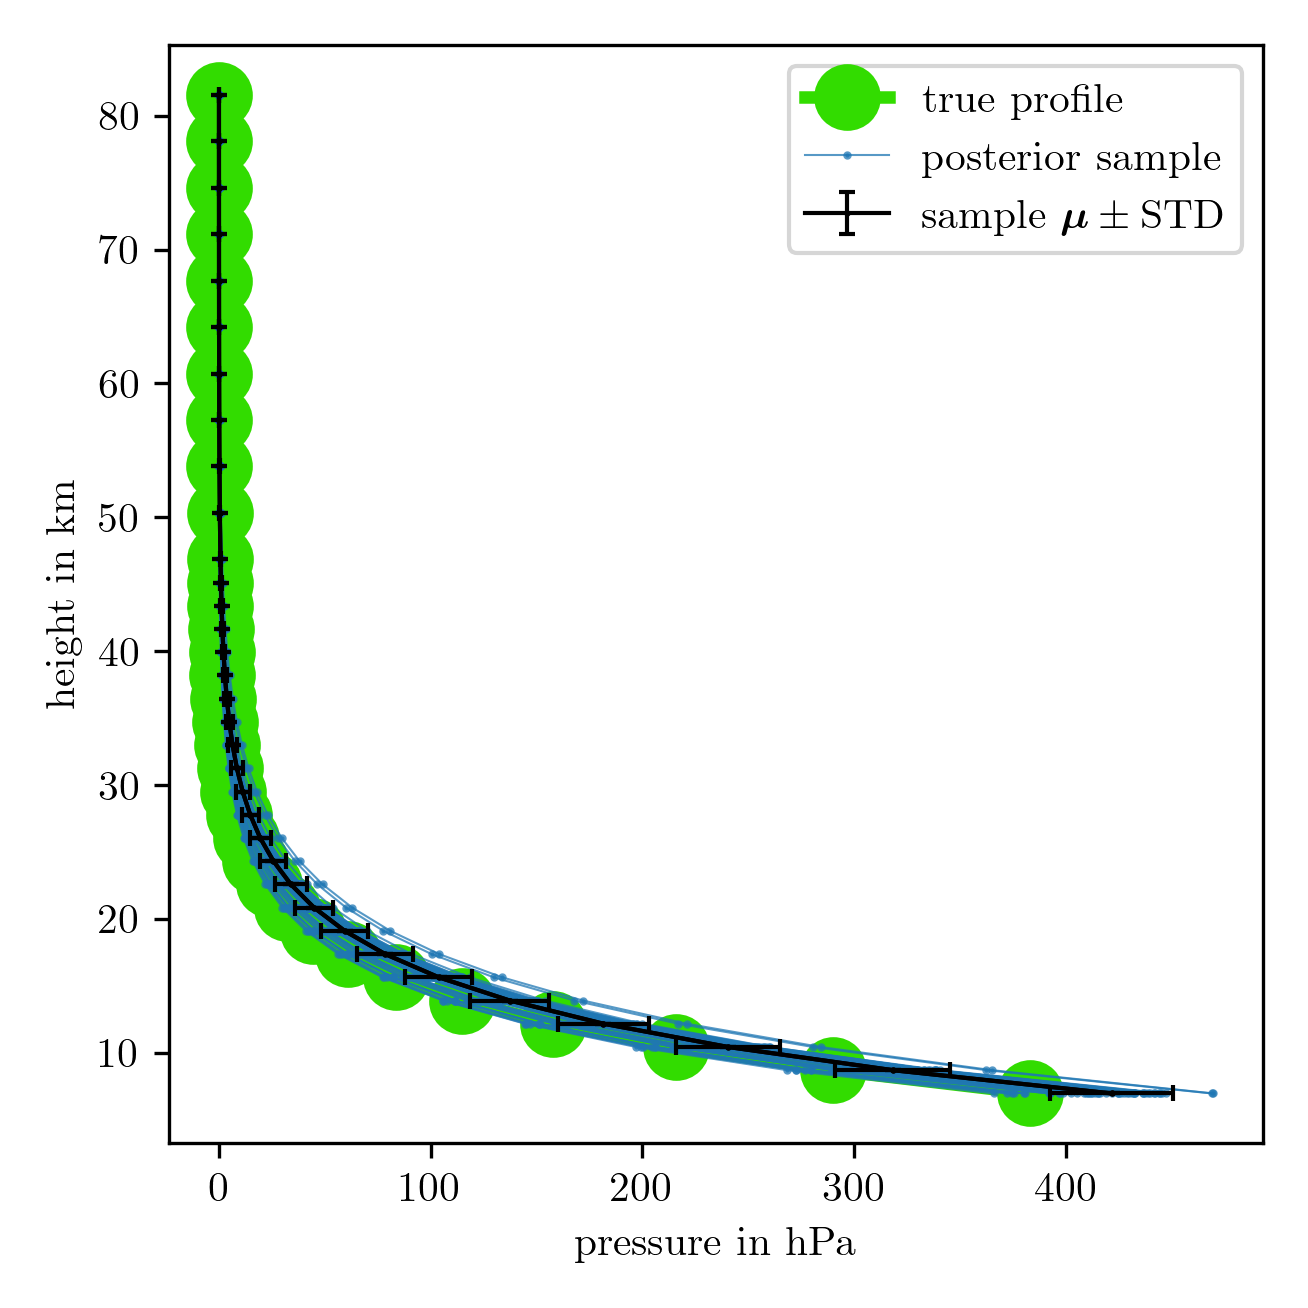
\includegraphics{PressPostMeanSigm.png}
	\caption[]{}
	\label{fig:}
\end{figure}



